%------------------------------------------------------------------------------
%	GENERAL FRAMEWORK
%------------------------------------------------------------------------------


\subsection{General Framework}

Conducting the literature review, it can be observed that, although \gls{AI}, and in particular \gls{DRL}, has a huge potential regarding the life-cycle optimization and maintenance of engineering systems, there are still considerable limitations. These limitations gave rise to the scope of the current project, and subsequently justify its future contribution.\\

To be more precise, the goal of the considered framework is to couple Bayesian Inference with \gls{DRL} algorithms, aiming to find the optimal sequence of maintenance actions for a stochastically deteriorating engineering system. The thought process, thus the motivation, behind the choice of these two core concepts is illustrated in Figure \ref{conceptFlowV1}.

\begin{figure}[H]
    \centering
	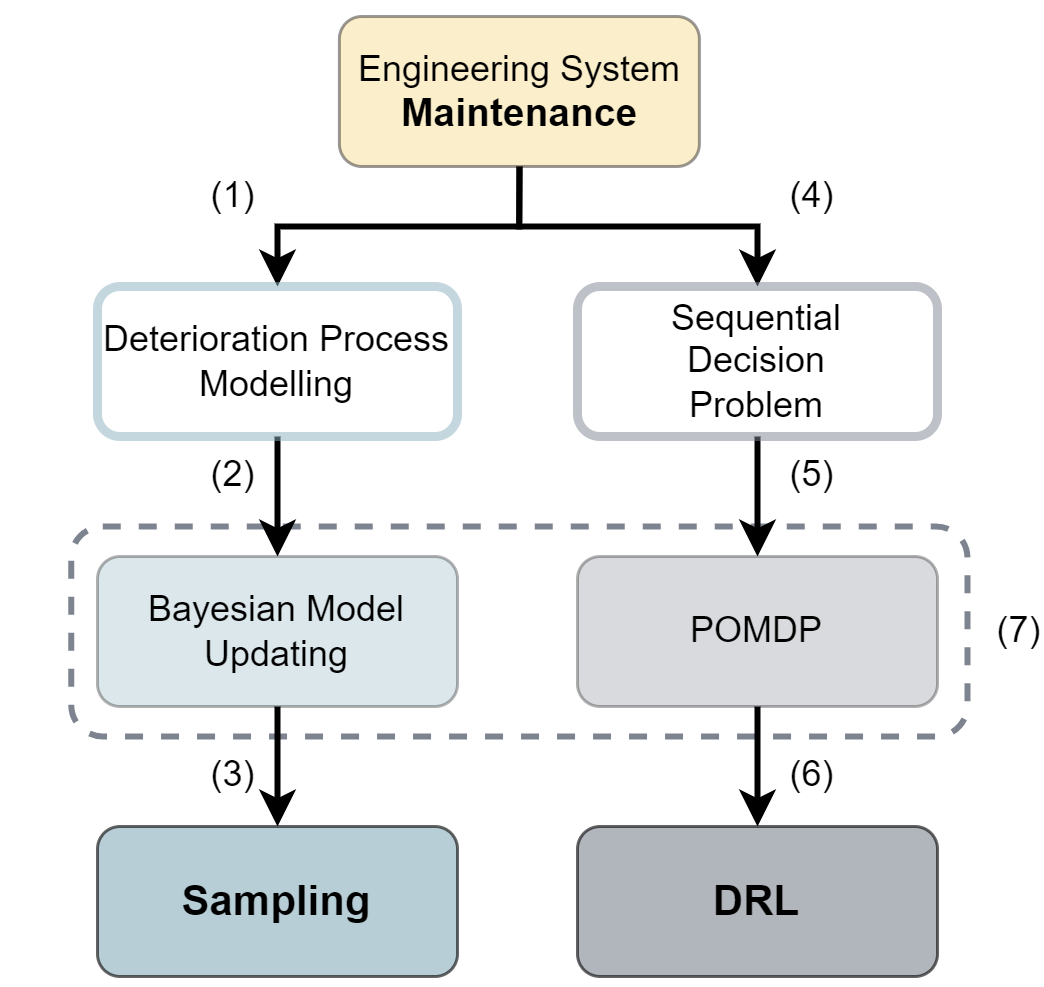
\includegraphics[width=0.6\linewidth]{Figures/conceptFlow.png}
	\caption{Problem conceptual breakdown - Motivation for the selected tools}
	\label{conceptFlowV1}
\end{figure}

In order to explain better this workflow, each logical step is numbered and further elaborated:



\begin{myEnum}
  \item A key concept interfering with any engineering system's maintenance, is its deterioration. As already stated, the way in which a system ages is not straightforward, since many uncertainties are involved in the physical degradation processes. Therefore, an important sub-problem constitutes the deterioration process modelling. 
  \item An efficient way to tackle the underlying stochasticity in the deterioration processes is to incorporate the ever-increasing available observed/measured data, in order to update the knowledge about the system's parameters; a key element in the \gls{BMU} concept.
  \item As explained in Section \ref{bmuSec}, applying Bayes Theorem (Equation \ref{bayesTheorem}), can be cumbersome, due to the inability to calculate the normalizing constant in the denominator, i.e. the so-called evidence $\prob{\boldsymbol{D}}$. This is the case especially in the inference of continuous variables, which justifies the choice of a sampling algorithm to tackle this obstacle.
  \item Returning to the general problem, the maintenance of an engineering system constitutes a sequential decision problem, since the sought strategy is defined by the optimal sequence of maintenance actions. 
  \item More often than not, \glspl{POMDP} are utilized since they provide a principled mathematical methodology for stochastic optimal control under uncertain action outcomes and observations \cite{morato2022optimal}.
  \item As elaborated in Chapter \ref{LitReview}, the most efficient way to solve a \gls{POMDP}, is \gls{DRL}, since it can handle multi-dimensionality, and even continuous state and action spaces, leading eventually to the wanted optimal strategy.
  \item It should be mentioned that both \gls{BMU} and \glspl{POMDP} rely on the same principles, employing Bayesian rules to update the system's parameters using observations in the former case, and update the state probability distribution, i.e. the so-called belief, in the latter one.
\end{myEnum}

The interaction between the different elements of the \gls{POMDP} for the current framework, i.e. beliefs, actions, rewards and observations, during each decision step, is depicted in Figure \ref{pomdpFig}. 

\begin{figure}[H]
    \centering
	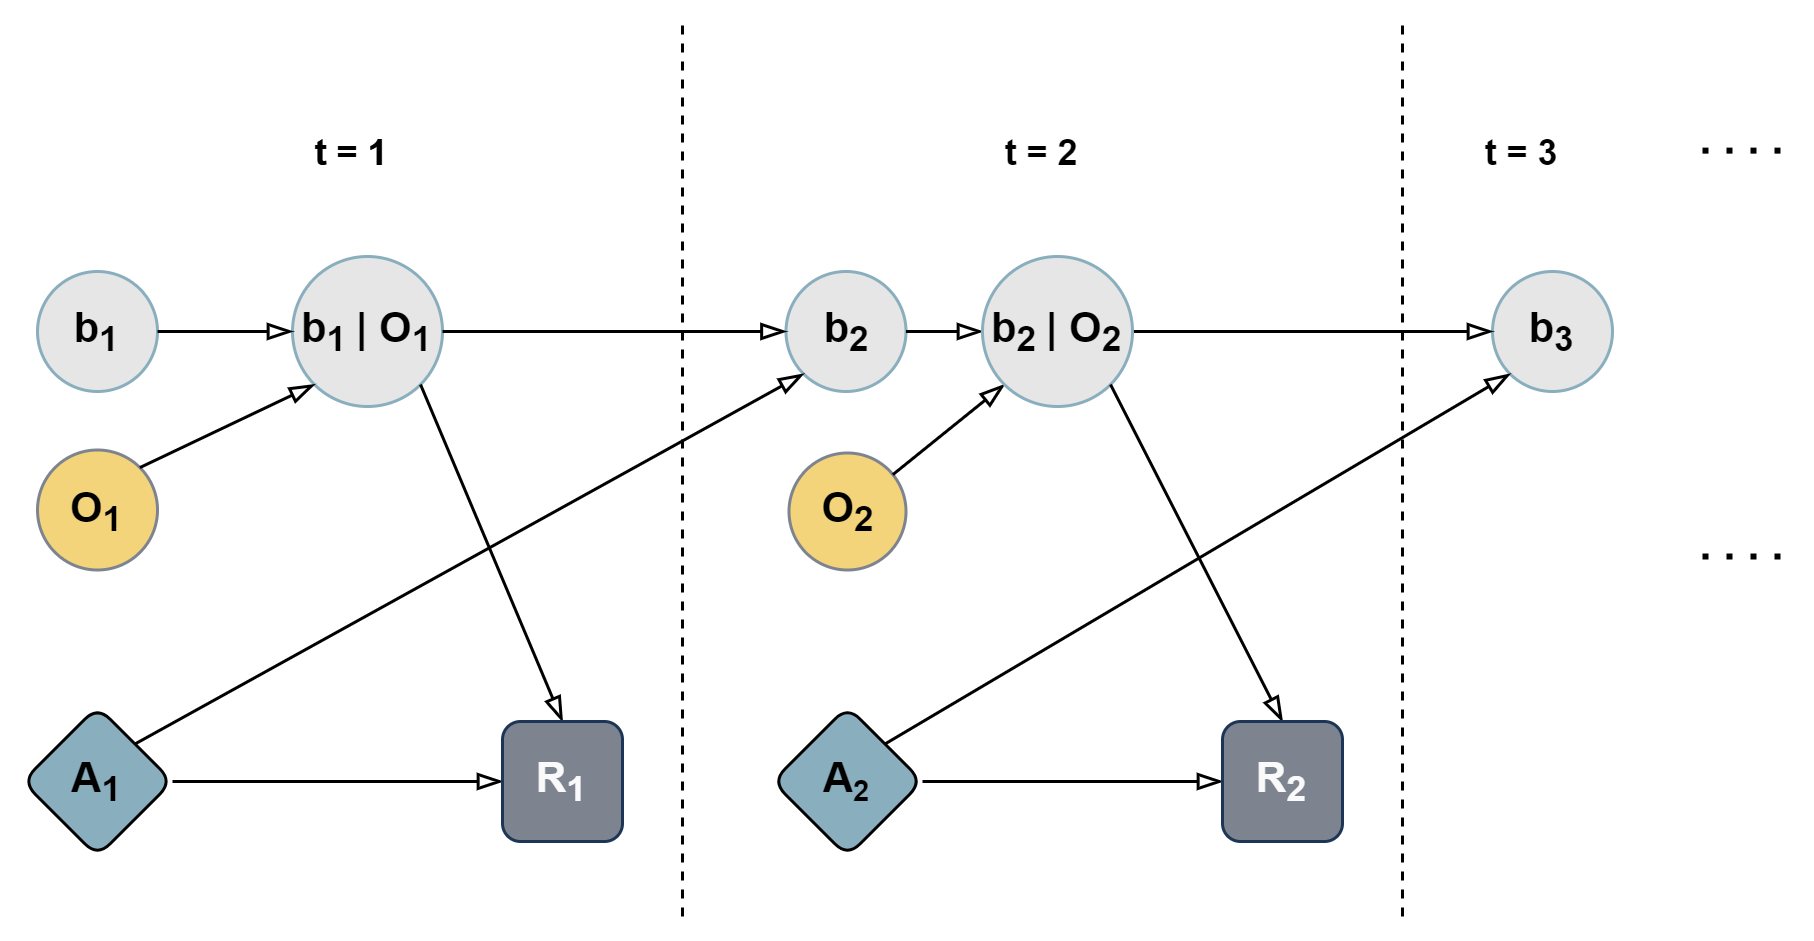
\includegraphics[width=0.8\linewidth]{Figures/pomdp.png}
	\caption{Graphical Model of the employed \acrshort{POMDP}}
	\label{pomdpFig}
\end{figure}

Elaborating in each of the components displayed in Figure \ref{pomdpFig}:

\begin{itemize}
    \item $\boldsymbol{b_t}$ is the unknown deterioration state. To be in accordance with the theory presented in Section \ref{pomdpSec}, it represents the belief, meaning a probability distribution about the deterioration of the system. On the contrary to the biggest part of the existing literature, where the deterioration space is discretized, in this project a continuous state-space is considered, hence, the belief is a continuous probability distribution.
    \item $\boldsymbol{O_t}$ is the observation that is obtained through a \gls{SHM} system periodically, i.e. in every decision step. This observation (possibly the acceleration at the location of the sensors) is fed into an \gls{OMA} scheme, in order to derive modal data, e.g. eigenfrequencies, eigenmodes, etc. It should be mentioned, that the \gls{OMA} step of this procedure will not be considered for the current project, since more emphasis is going to be given on the \gls{DRL} and \gls{BMU} parts. Therefore, the needed modal data will be generated directly, taking into account that they are contaminated with noise. 
    \item $\boldsymbol{A_t}$ is the maintenance action that is taken at the decision step, $t$. The action space is assumed to be discrete.
    \item $\boldsymbol{R_t}$ is the reward received for taking the action $A_t$ when in state $S_t$. As displayed in Sections \ref{mdpSec} and \ref{pomdpSec}, the expected return of the sum of these rewards, including also a discounting factor $\gamma$ for future rewards, is the quantity that needs to be maximized (Equation \ref{expReturn}). In the current project, the rewards correspond to the costs, thus, the goal is the minimization of the rewards. At any given state, the reward/cost can be decomposed into two sub-costs, i.e. the cost of the taken action and the cost associated with the risk of failure.\\
    \begin{equation}
        R_t = C_t = C_{A_t} + C_{\text{risk}} \label{rewardEq}
    \end{equation}
    The risk of failure cost is calculated as the product of the probability of failure times the failure cost, i.e. $C_{\text{risk}} = P_f \cdot C_F$. An important matter constitutes the calculation of this probability for every deterioration state. 
    \item $\boldsymbol{b_t \mid O_t}$ is the updated deterioration state, having included the information of the observation $O_t$. This means that at every decision step, a Bayesian Inference is performed in order to improve the knowledge, i.e. the probability distribution, about the deterioration parameters of interest. The updating is executed using the \gls{NUTS} method, which will be briefly introduced in the coming section (Section \ref{nutsSec}).
\end{itemize}

\newpage

The proposed general framework is illustrated in more detail in Figure \ref{genFlow}.

\begin{figure}[H]
    \centering
	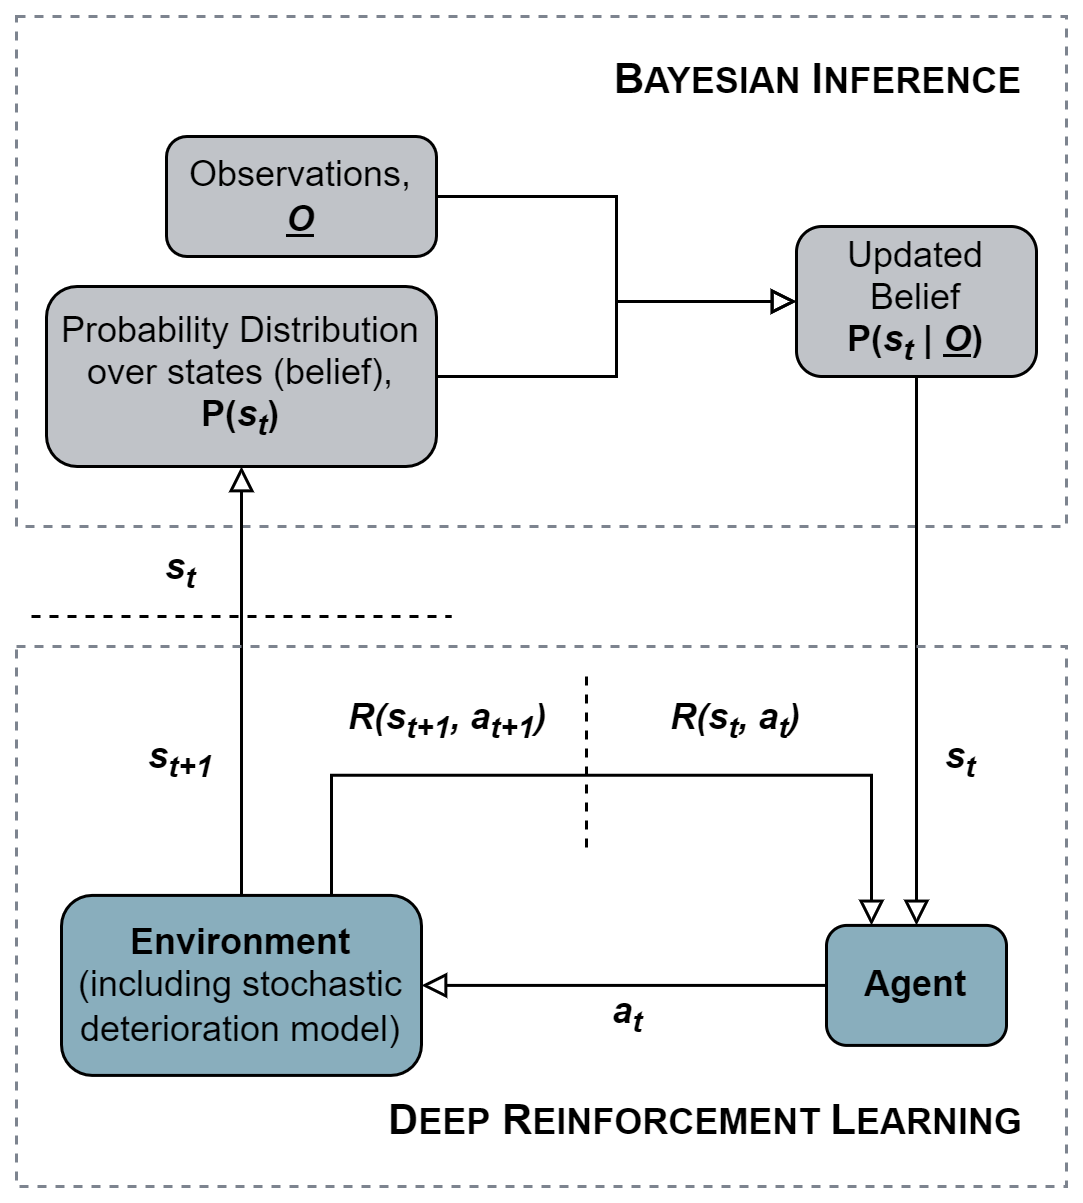
\includegraphics[width=0.54\linewidth]{Figures/generalFlow.png}
	\caption{Proposed Framework}
	\label{genFlow}
\end{figure}


%------------------------------------------------------------------------------
%	SAMPLING ALGORITHM
%------------------------------------------------------------------------------


\subsection{Sampling Algorithm} \label{nutsSec}

For the sake of completeness and transparency regarding the proposed framework, a brief walkthrough the sampling procedure used, is presented in this section. To be more precise, the chosen sampling method is \gls{NUTS}, which will be applied through the probabilistic programming \verb|Python| package of \verb|PyMC3| \cite{salvatier2016probabilistic}.\\

As already mentioned, in bayesian inference problems the posterior distribution is usually intractable. The commonly used \gls{MCMC} methods, approach the target distribution by drawing a series of correlated samples. However, in complicated problems with many parameters, widely applicable methods such as random-walk Metropolis and Gibbs sampling, could be computationally expensive to achieve convergence, because of the random walks with which they explore the parameter space. This is why, in applications with continuous model parameters \gls{HMC} has been proven more efficient, shifting from a problem of sampling to a problem of simulating Hamiltonian dynamics, as elaborated in \cite{neal2011mcmc}. \\

Nevertheless, in order to apply \gls{HMC} there are two tuning parameters that the user needs to calibrate, i.e. the step size $\epsilon$ and the number of steps $L$ for which the simulated Hamiltonian system is ran. Determining these parameters is usually a cumbersome and time-efficient task, that requires also some experience, which is the reason why \gls{HMC} is not widely used. Nonetheless, it provides the foundation for \gls{NUTS}, which is a self-tuning algorithm that eliminates the need to choose the problematic number-of-steps parameter $L$. At the same time, the version of \gls{NUTS} which will be used through \verb|PyMC3|, includes a dual averaging scheme, introduced in \cite{nesterov2009primal}, which automatically tunes the step size parameter $\epsilon$, too.\\

As it exceeds the scope of the current research, more information about the exact mathematical formulation of both \gls{HMC} and \gls{NUTS}, as well as the step by step algorithms, are presented in \cite{hoffman2014no}. However, the main algorithms are presented briefly along with the core principles, as elaborated on the aforementioned paper.\\

In \gls{HMC} an auxialiary momentum variable $r_d$ is introduced for the model variables $\theta_d$, which are usually drawn independently from the standard normal distribution, leading to their joint density being:

\begin{equation}
    \prob{\theta, r} \propto \exp \big\{ \ccal{L} (\theta) - 0.5\, r\cdot r\big\}
\end{equation}

\blfootnote{Even though $\theta$ and $r$ are vectors, they are not underlined (which would be consistent with the thesis' notation) in order to be in accordance with the original paper \cite{hoffman2014no}}

where $\ccal{L}$ is the logarithm of the joint density of the values of interest $\theta$, while $r \cdot r$ denotes the inner product between the momentum vectors. \\

A fictitious Hamiltonian system can be used instead of this augmented model, where each parameter gains a physical meaning. In particular, $\theta$ corresponds to the particle's position in the $D$-dimensional space, $r$ denotes its momentum, $\ccal{L}$ is the negative potential energy function for the given position, $0.5\,r\cdot r$ is the particle's kinetic energy and lastly $\log \prob{\theta, r}$ is the negative energy of the particle. The evolution over time of this Hamiltonian system, is often simulated through the St\"{o}rmer-Verlet (``leapfrog'') integrator, which is presented in Algorithm \ref{alg1NutsPaper}.\\

\begin{algorithm}[H]
    \caption{St\"{o}rmer-Verlet (``leapfrog'') integrator}
    \label{alg1NutsPaper}
    \SetKwProg{leapFrogFunc}{Leapfrog}{:}{}
    \leapFrogFunc{($\theta, r, \epsilon$)}{
        Set $\Tilde{r} \gets r + (\epsilon / 2) \, \nabla _{\theta} \ccal{L}(\theta)$\\
        Set $\Tilde{\theta} \gets \theta + \epsilon\, \Tilde{r}$\\
        Set $\Tilde{r} \gets \Tilde{r} + (\epsilon / 2) \, \nabla _{\theta} \ccal{L}(\Tilde{\theta})$\\
        \Return $\Tilde{\theta}, \Tilde{r}$
    }
    
\end{algorithm}

\newpage

Having introduced the basic principles, the complete \gls{HMC} algorithm is presented in Algorithm \ref{hmcAlgo}.\\

\begin{algorithm}[H]
    \caption{\acrfull{HMC}}
    \label{hmcAlgo}
    \SetKw{leap}{Leapfrog}
    
    Given $\theta^0, \, \epsilon, \, L,\,\ccal{L},\, M$
    \For{$m=1$ \KwTo $M$}{
        Sample $r^0 \sim \ccal{N}(0, I)$ \tcp{$I$ denotes the identity matrix}\\
        Set $\theta ^m \gets \theta ^{m-1},\,\Tilde{\theta}\gets \theta ^{m-1},\,\Tilde{r} \gets r^0$\\
        \For{$i=1$ \KwTo $L$}{
            Set $\Tilde{\theta}, \Tilde{r} \gets \leap(\Tilde{\theta}, \Tilde{r}, \epsilon)$
        }
        With probability $\alpha = \min \bigg\{ 1, \cfrac{\exp \left( \ccal{L} (\Tilde{\theta})-0.5\, \Tilde{r}\cdot \Tilde{r} \right)}{\exp \left( \ccal{L} (\theta^{m-1})-0.5\, r^0 \cdot r^0\right) } \bigg\}$, set $\theta^m \gets \Tilde{\theta}, \, r^m \gets - \Tilde{r}$
    }
\end{algorithm}

\vspace{0.5cm}

where $L$ is the number of steps, i.e. Leapfrog updates, and $M$ is the amount of drawn samples.\\

\newpage

As mentioned already, a crucial improvement on \gls{HMC} is the self-tuning of the hyperparameters, $\epsilon$ and $L$, which is being done by the \gls{NUTS} algorithm. To determine when the amount of leapfrog steps is sufficient, a recursive function is used, namely \textit{Buildtree}, which is presented in Algorithm \ref{algBuildTreeNutsPaper}.\\


\begin{algorithm}[H]
    \cprotect\caption{BuildTree\footnotemark recursive function}
    \label{algBuildTreeNutsPaper}
    \SetKwProg{buildFun}{BuildTree}{:}{}
    \SetKw{leap}{Leapfrog}
    \SetKw{buildKw}{BuildTree}
    
    \buildFun{($\theta,\, r,\, u,\, v,\, j,\, \epsilon,\, \theta ^0,\, r^0$)}{
        \If{$j=0$}{
            \textit{Base case - take one leapfrog step in the direction $v$}\\
            $\theta ^{\prime},\, r^{\prime} \gets \leap (\theta,\, r,\, v\,\epsilon)$\\
            $n^{\prime} \gets \mathds{I}\bigg[ u\leq \exp \big\{ \ccal{L}(\theta ^{\prime}) - 0.5\, r^{\prime}\cdot r^{\prime}\big\}\bigg]$\\
            $s^{\prime} \gets \mathds{I}\bigg[ u< \exp \big\{ \Delta _{\max} + \ccal{L}(\theta ^{\prime}) - 0.5\, r^{\prime}\cdot r^{\prime}\big\}\bigg]$\\
            \Return $\theta ^{\prime},\, r^{\prime},\,\theta ^{\prime},\, r^{\prime},\,\theta^{\prime},\, n^{\prime},\, s^{\prime},\, \min \bigg\{ 1, \exp \big\{ \ccal{L}(\theta^{\prime}) - 0.5\, r^{\prime} \cdot r^{\prime} - \ccal{L}(\theta ^0) + 0.5\, r^0\cdot r^0 \big\} \bigg\},\, 1 $
        }
        \Else{
            \textit{Recursion - implicitly build the left and right subtrees}\\
            $\theta ^-,\, r^-,\, \theta ^+,\, r^+,\, \theta ^{\prime},\, n^{\prime},\, s^{\prime},\,\alpha^{\prime},\, n^{\prime}_{\alpha} \gets \buildKw (\theta,\, r,\,u,\, v,\, j-1,\, \epsilon,\,\theta^0,\, r^0)$\\
            \If{$s^{\prime}=1$}{
                \If{$v=-1$}{
                    $\theta ^-,\, r^-,\,-,\, -,\, \theta ^{\prime\prime},\, n^{\prime\prime},\, s^{\prime\prime},\,\alpha^{\prime\prime},\, n^{\prime\prime}_{\alpha} \gets \buildKw (\theta^-,\, r^-,\,u,\, v,\, j-1,\, \epsilon,\,\theta^0,\, r^0)$
                }
            \Else{
                $-,\, -,\, \theta ^+,\, r^+,\, \theta ^{\prime\prime},\, n^{\prime\prime},\, s^{\prime\prime},\,\alpha^{\prime\prime},\, n^{\prime\prime}_{\alpha} \gets \buildKw (\theta^+,\, r^+,\,u,\, v,\, j-1,\, \epsilon,\,\theta^0,\, r^0)$
            }
            With probability $\cfrac{n^{\prime\prime}}{n^{\prime} + n^{\prime\prime}}$, set $\theta ^{\prime} \gets \theta ^{\prime\prime}$\\
            Set $\alpha ^{\prime} \gets \alpha ^{\prime} + \alpha ^{\prime\prime}, \, n^{\prime}_{\alpha} \gets n^{\prime}_{\alpha} + n^{\prime\prime}_{\alpha}$\\
            $s^{\prime} \gets s^{\prime\prime} \, \mathds{I}\bigg[ (\theta ^+ - \theta ^-) \cdot r^- \geq 0 \bigg] \, \mathds{I}\bigg[(\theta ^+ - \theta ^-) \cdot r^+ \geq 0 \bigg]$\\
            $n^{\prime} \gets n^{\prime} + n^{\prime\prime}$
            }
        \Return $\theta ^-, \, r^-, \, \theta ^+, \, r^+,\, \theta ^{\prime}, \, n^{\prime},\, s^{\prime},\, \alpha ^{\prime}, \, n^{\prime}_{\alpha}$
        }
    }
\end{algorithm}

\footnotetext{More information on the \textit{BuildTree} function, its input, output and intermediate steps, can be found in \cite{hoffman2014no}.}

\vspace{0.5cm}

where $\mathds{I}[\cdot ]$ is a boolean operator, returning $1$ if the expression inside brackets is true, and $0$ if false.

\newpage

As far as the choice of $\epsilon$ is concerned, the function used and the step by step procedure is presented in Algorithm \ref{alg4NutsPaper}.\\

\begin{algorithm}[H]
    \caption{Heuristic for choosing an initial value of $\epsilon$}
    \label{alg4NutsPaper}
    \SetKwProg{epsFun}{FindReasonableEpsilon}{:}{}
    \SetKw{leap}{Leapfrog}
    \epsFun{($\theta$)}{
        Initialize $\epsilon = 1, \, r\sim \ccal{N}(0, I)$ \tcp{$I$ denotes the identity matrix}\\
        Set $\theta^{\prime}, r^{\prime} \gets$ \leap ($\theta, r, \epsilon$)\\
        $a \gets 2 \, \mathds{I} \bigg[ \cfrac{\prob{\theta^{\prime}, r^{\prime}}}{\prob{\theta, r}} > 0.5 \bigg] -1 $\\
        \While{$\big ( \cfrac{\prob{\theta^{\prime}, r^{\prime}}}{\prob{\theta, r}} \big ) ^ a > 2 ^{-a}$}{
            $\epsilon \gets 2^a\,\epsilon$\\
            Set $\theta ^{\prime}, r^{\prime} \gets \leap (\theta, r, \epsilon)$
        }
        \Return $\epsilon$
    }
\end{algorithm}


\newpage 

Moving towards the final algorithm which is followed by the \verb|PyMC3| package, Algorithm 6 of \cite{hoffman2014no}, namely \acrfull{NUTS} with Dual Averaging, is presented in Algorithm \ref{alg6NutsPaper} of the current project.\\

\begin{algorithm}[H]
    \caption{\acrfull{NUTS} with Dual Averaging}
    \label{alg6NutsPaper}
    \SetKw{findEps}{FindReasonableEpsilon}
    \SetKw{buildKw}{BuildTree}
    \SetKw{leap}{Leapfrog}
    
    Given $\theta ^0, \delta, \ccal{L}, M, M^{\text{adapt}}$\\
    Set $\epsilon _0 = \findEps (\theta), \, \mu = \log (10\, \epsilon _0), \, \bar{\epsilon}_0 = 1, \, \bar{H}_0 = 0, \, \gamma = 0.05, \, t_0 = 10, \, \kappa = 0.75$\\
    \For{$m=1$ \KwTo $M$}{
        Sample $r^0 \sim \ccal{N}(0, I)$\\
        Resample $u \sim \mathrm{Uniform}\bigg(\big[0, \exp \big\{ \ccal{L}(\theta ^{m-1} - 0.5\, r^0 \cdot r^0)\big\}\big]\bigg)$ \\
        Inititalize $\theta ^- = \theta ^{m-1}, \, \theta ^+ = \theta ^{m-1}, \, r^- = r^0,\, r^+ = r^0, \, j=0,\, \theta ^m = \theta ^{m-1},\, n =1 ,\, s=1$\\
        \While{s=1}{
            Choose a direction $v_j \sim \mathrm{Uniform}(\{-1, 1\})$\\
            \If{$v_j=-1$}{
                $\theta ^-,\, r^-,\, -,\, -,\, \theta ^{\prime},\, n^{\prime},\, s^{\prime},\,\alpha,\, n_{\alpha} \gets \buildKw (\theta ^-,\, r^-,\,u,\, v_j,\, j,\, \epsilon_{m-1},\,\theta^{m-1},\, r^0)$
            }
            \Else{
                $-,\, -,\, \theta ^+,\, r^+,\, \theta ^{\prime},\, n^{\prime},\, s^{\prime},\,\alpha,\, n_{\alpha} \gets \buildKw (\theta ^+,\, r^+,\,u,\, v_j,\, j,\, \epsilon_{m-1},\,\theta^{m-1},\, r^0)$
            }
            \If{$s^{\prime} = 1$}{
                With probability $\min \big\{1, \cfrac{n^{\prime}}{n}\big\}$, set $\theta ^m \gets \theta ^{\prime}$
            }
            $n \gets n + n^{\prime}$\\
            $s \gets s^{\prime} \, \mathds{I}\big[ (\theta ^+ - \theta ^-) \cdot r^- \geq 0 \big]\, \mathds{I}\big[ (\theta ^+ - \theta ^-) \cdot r^+ \geq 0 \big] $\\
            $j \gets j +1$
        }
        \If{$m\leq M^{\text{adapt}}$}{
            Set $\bar{H}_m = \bigg( 1 - \cfrac{1}{m + t_0} \bigg)\, \bar{H}_{m-1} + \cfrac{1}{m+t_0}\,\big(\delta - \cfrac{\alpha}{n_{\alpha}}\big)$\\
            Set $\log \epsilon _m = \mu - \cfrac{\sqrt{m}}{\gamma}\, \bar{H}_m,\, \log \bar{\epsilon}_m = m ^{-\kappa}\, \log \epsilon _m + (1 - m^{-\kappa}) \, \log \bar{\epsilon}_{m-1}$
        }
        \Else{
            Set $\epsilon _m = \bar{\epsilon}_{M^{\text{adapt}}}$
        }
    }
\end{algorithm}

\vspace{0.5cm}

where $\delta$ is the desired average acceptance probability of the samples and $M^{\text{adapt}}$ is the number of iterations after which the adaption is stopped.


\newpage

%------------------------------------------------------------------------------
%	DRL ALGORITHMS
%------------------------------------------------------------------------------

\subsection{\acrfull{DRL} algorithms}

It has already been mentioned that in \gls{DRL} the value functions $Q, V$ as well as the policy $\pi$ are approximated by a \gls{DNN}, in order not only to capture efficiently their non-linear behaviour, but also, achieve a reparameterization, and express them in terms of the network's weights, so as to decrease the computational cost and instabilities.\\

An illustration of such networks is displayed in Figure \ref{dnnArchitectures}. The input to the \gls{DNN} is the state (or belief\footnotemark), $s_t$, while the output layer includes the action-state value function for every possible action, $a_t \in \ccal{A}$, in the case of \gls{DQN} and \gls{DDQN}. In a similar fashion for actor-critic algorithms like \gls{A2C} and \gls{PPO}, the actor and the critic neural networks are illustrated in Figures \ref{actorNet}, \ref{criticNet}. The former takes as input the state and yields as an output the probability to take each action given the state, $\pi(a_t \mid s_t)$, and the later using the same input, i.e. the state, returns the corresponding value state function, $V(s_t)$.\\

\footnotetext{The used $s_t$ notation represents the belief vector $\underline{b}$ along with any other input quantities (e.g. age) that together compose the state, and are passed as input to the neural networks.}

\begin{figure}[H]
    \centering
    \begin{subfigure}[b]{0.7\textwidth}
        \centering
        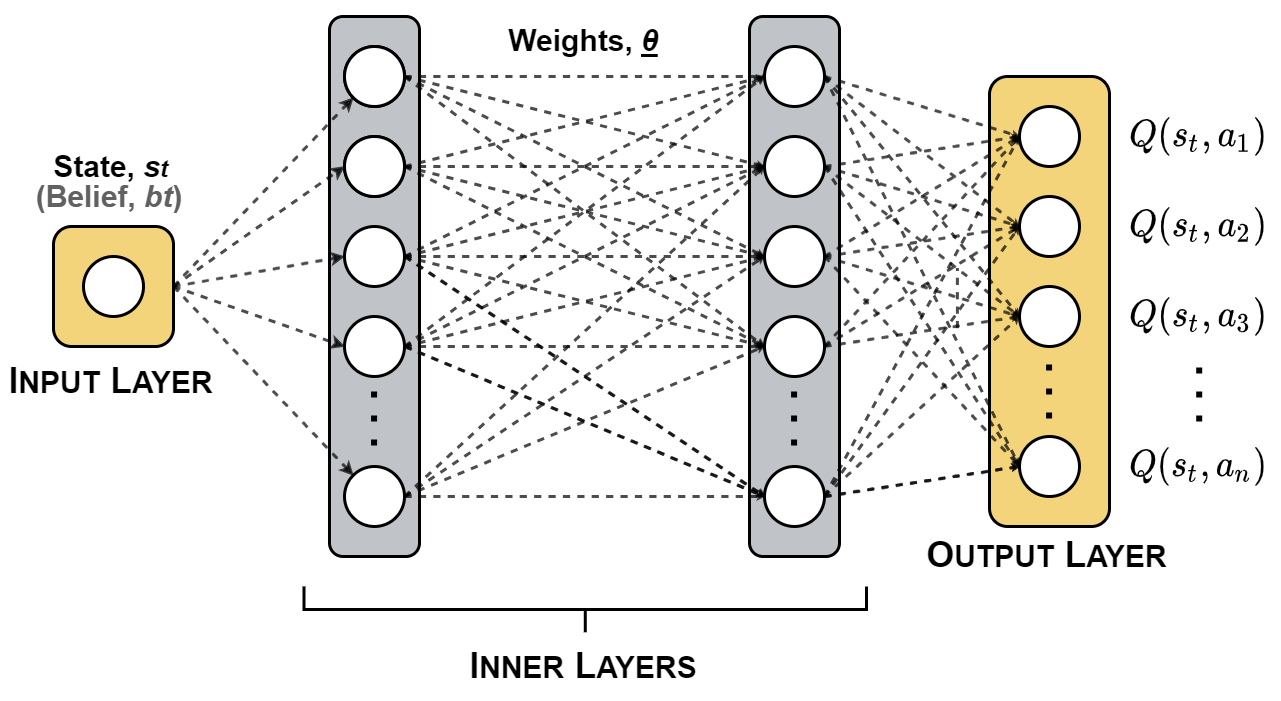
\includegraphics[width=\textwidth]{Figures/formalDNN.png}
        \caption{\gls{DQN}/\gls{DDQN} approximating the Q-function}
        \label{ddqnNet}
    \end{subfigure}
    \begin{subfigure}[b]{0.48\textwidth}
        \centering
        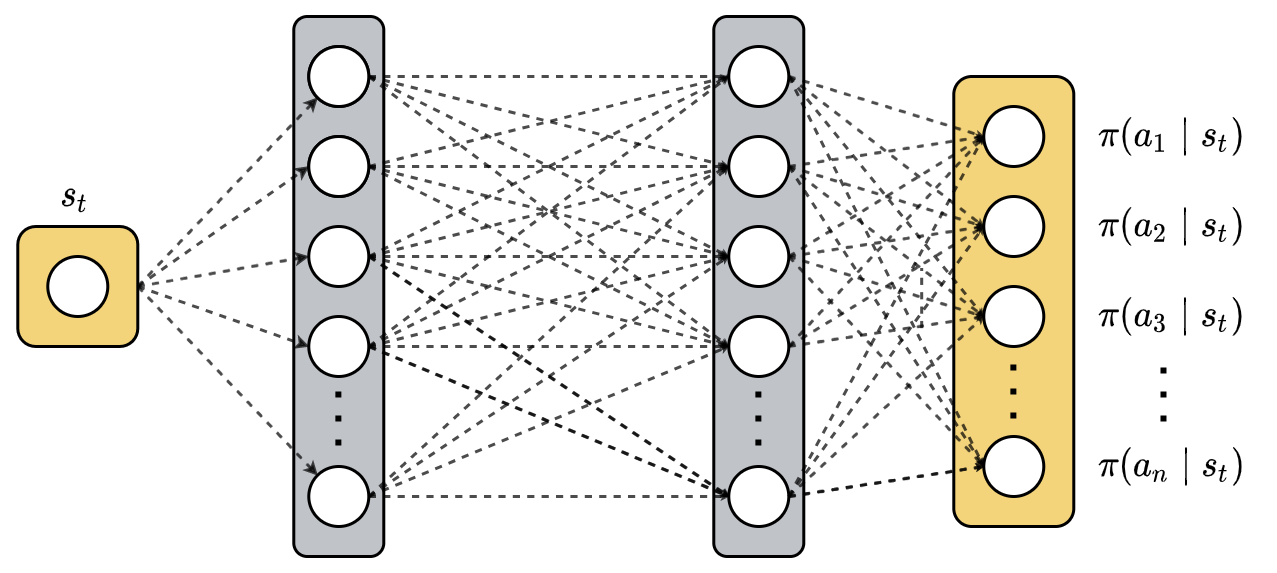
\includegraphics[width=\textwidth]{Figures/actorNet.png}
        \caption{Actor neural network}
        \label{actorNet}
    \end{subfigure}
    \hfill
    \begin{subfigure}[b]{0.48\textwidth}
        \centering
        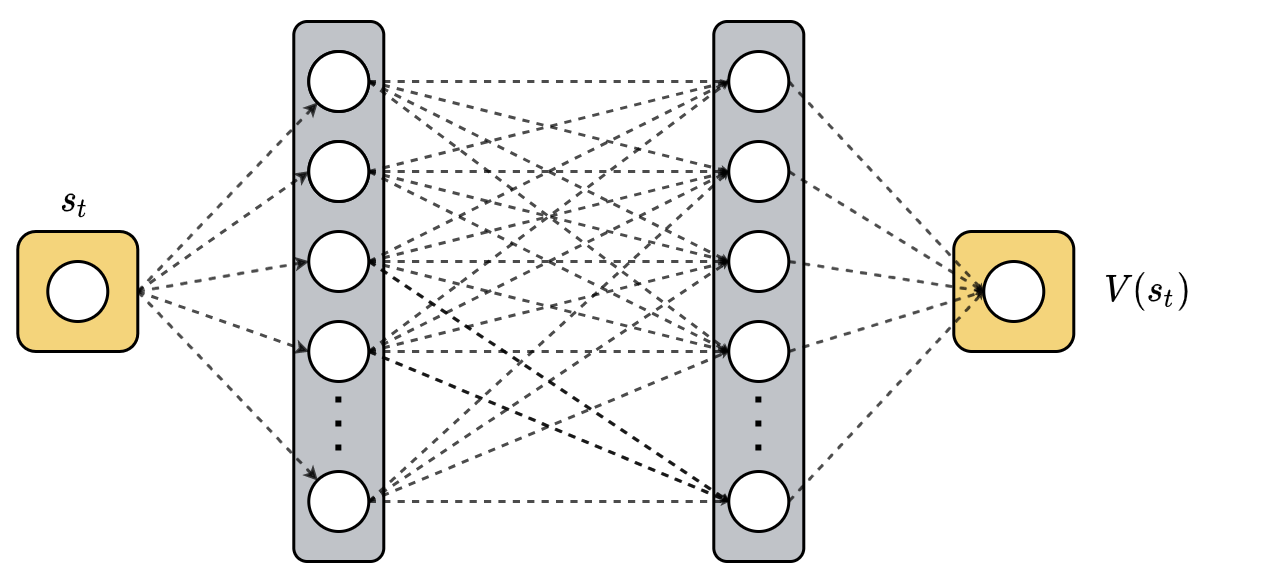
\includegraphics[width=\textwidth]{Figures/ctiricNet.png}
        \caption{Critic neural Network}
        \label{criticNet}
    \end{subfigure}
    \caption{Actor-critic \gls{DNN} architectures \protect\footnotemark}
    \label{dnnArchitectures}
\end{figure}

\footnotetext{The amount of inner layers and neurons depicted is for the sake of a more clear and explanatory representation}

\newpage

The \gls{DRL} algorithms that will be considered in the current project are:
\begin{itemize}
    \item \acrfull{DDQN}
    \item \acrfull{A2C}
    \item \acrfull{PPO}
\end{itemize}

The step-by-step procedure for all three of them, as found in literature, is described in the following subsections and more specifically in Algorithms \ref{DDQNalgo}, \ref{A2Calgo}, \ref{PPOalgo}, respectively.\\

%------------------------------------------------------------------------------
%	DOUBLE DEEP Q-NETWORK
%------------------------------------------------------------------------------

\subsubsection{\acrfull{DDQN}} \label{ddqnSec}

\begin{algorithm}[H]
    \caption{\acrfull{DDQN}}
    \label{DDQNalgo}
    Initialize primary network weights $\theta$\\
    Initialize target network weights $\theta^{-}$\\
    Initialize replay buffer\\
    Set target update time $T_{\text{update}}$\\
    \For {$episode \gets 1$ \KwTo $M$}{
        \For {$t \gets 1$ \KwTo $T$}{
            Select action $a_t$ according to $\epsilon$-greedy method\\
            Collect reward $R(s_t, a_t)$, observe next state $s_{t+1}$\\
            Store tuple $\left( s_t, a_t, R(s_t,a_t), s_{t+1} \right)$ in replay buffer\\
            Sample batch of tuples $\left( s_i, a_i, R(s_i,a_i), s_{i+1} \right)$ from replay buffer\\
            \If{$s_{i+1}$ is terminal state}{$y_i = R(s_i, a_i)$}
            \Else{$y_{t}=R(s_{t}, a_{t})+\gamma \,Q\left(s_{t+1}, \arg \max Q\left(s_{t+1}, a_{t+1} \mid \theta \right) \mid \theta^- \right)$}
            Update parameters $\theta$ according to: $\nabla_{\theta} L\left(\theta \right) \simeq \sum \left[\left( Q\left(s_i, a_i \mid \theta \right) -y_i \right) \nabla_{\theta} Q\left(s_i, a_i \mid \theta \right)\right]$\\
            \If{$T_{\text{update}}$}{$\theta ^- = \theta$} 
        }
    }
\end{algorithm}

%------------------------------------------------------------------------------
%	ADVANTAGE ACTOR CRITIC
%------------------------------------------------------------------------------

\subsubsection{\acrfull{A2C}} \label{a2cSec}

\begin{algorithm}[H]
    \caption{\acrfull{A2C}}
    \label{A2Calgo}
    Initialize policy parameters $\theta $\\
    Initialize value function parameters $\theta _v$\\
    \For {$Episode=0,1,2 \ldots$}{
        \For{$t \gets 1$ \KwTo $T$}{
            Perform $a_t$ according to policy $\pi(a_t\mid s_t, \theta)$\\
            Collect reward $R(s_t, a_t)$, observe next state $s_{t+1}$\\
        }
        \If{terminal $s_t$}{$R=0$}
        \Else{$R=V(s_t\mid \theta _v)$\tcp{Bootstrap from last state}}
        Update $\theta$ according to: 
        $$\nabla _{\theta} J(\theta) = \mathbb{E}_{s_t,a_t}\left[ \sum _{t\geq 0} \nabla _{\theta} \log \pi (a_t \mid s_t, \theta) \, \left( R(s_t, a_t) + \gamma \, V(s_{t+1} \mid \theta _v) - V(s_t \mid \theta _v) \right) \right] $$\\
        Update $\theta _v$ according to:
        $$\nabla _{\theta_v} J(\theta_v) = \mathbb{E}_{s_t,a_t}\left[ \nabla _{\theta _v}V(s_t \mid \theta _v) \, \left( R(s_t, a_t) + \gamma \, V(s_{t+1}\mid \theta _v) - V(s_t\mid \theta _v) \right) \right]$$
    }
\end{algorithm}

%------------------------------------------------------------------------------
%	PROXIMAL POLICY OPTIMIZATION
%------------------------------------------------------------------------------

\subsubsection{\acrfull{PPO}} \label{ppoSec}

\begin{algorithm}[H]
    \caption{\acrfull{PPO} \cite{PPOspinningup}}
    \label{PPOalgo}
    Initialize policy parameters $\theta _0$\\
    Initialize value function parameters $\phi _0$\\
    \For {$k=0,1,2 \ldots$}{
        Collect set of trajectories $\ccal{D}_k=\{\tau_i\}$ by running policy $\pi _k = \pi(\theta _k)$ in the environment\\
        Compute rewards-to-go $R_t$\\
        Compute advantage estimates, $A_t$ (using any method of advantage estimation) based on the current value function $V_{\phi_k}$\\
        Update the policy by maximizing the \gls{PPO}-Clip objective:
        $$\theta_{k+1}=\arg \max _{\theta} \cfrac{1}{\left|\ccal{D}_{k}\right| T} \sum_{\tau \in \ccal{D}_{k}} \sum_{t=0}^{T} \min \left(\cfrac{\pi_{\theta}\left(a_{t} \mid s_{t}\right)}{\pi_{\theta_{k}}\left(a_{t} \mid s_{t}\right)} A^{\pi_{\theta_{k}}}\left(s_{t}, a_{t}\right), \quad g\left(\epsilon, A^{\pi_{\theta_{k}}}\left(s_{t}, a_{t}\right)\right)\right)$$
        typically via stochastic gradient ascent with Adam\\
        Fit the value function by regression on mean-squared error:
        $$\phi_{k+1}=\arg \min _{\phi} \cfrac{1}{\left|\ccal{D}_{k}\right| T} \sum_{\tau \in \ccal{D}_{k}} \sum_{t=0}^{T}\left(V_{\phi}\left(s_{t}\right)-R_{t}\right)^{2}$$
        typically via some gradient descent algorithm
    }
\end{algorithm}

\newpage

\subsection{Conclusions}

Having elaborated on the selected algorithms of this project, an updated version of the conceptual breakdown flowchart (Figure \ref{conceptFlowV1}) is illustrated in Figure \ref{concFlow2}.

\begin{figure}[H]
    \centering
	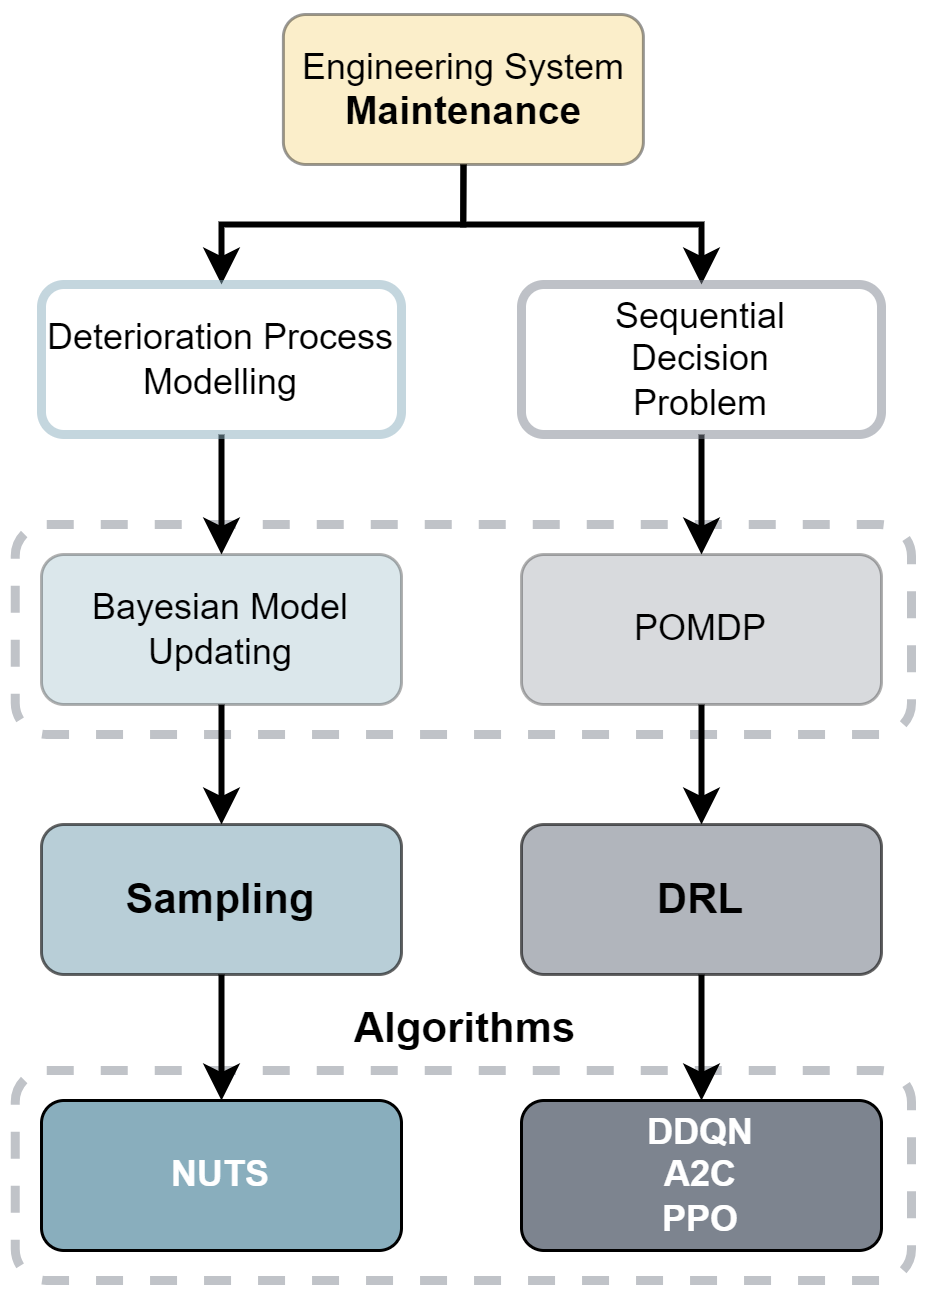
\includegraphics[width=0.5\linewidth]{Figures/conceptFlowV2.png}
	\caption{Problem conceptual breakdown - Motivation for the selected tools and algorithms}
	\label{concFlow2}
\end{figure}

This flowchart acts both as a summary of the current chapter as well as the motivation and reasoning behind the choice of the specific algorithms. It moves from the general problem to be tackled, namely ``Engineering System Maintenance'', to the most efficient tools existent for every sub-task, i.e. \gls{NUTS}, \gls{DDQN}, \gls{A2C} and \gls{PPO}.